\renewcommand{\theequation}{\theenumi}
\begin{enumerate}[label=\thesubsection.\arabic*.,ref=\thesubsection.\theenumi]
\numberwithin{equation}{enumi}

\item The general of a circle equation is $\norm{\vec{x}-\vec{O}} = r$.
\begin{align}
\norm{\vec{x}-\vec{O}}^2 &= r^2 \\
\implies \brak{\vec{x}-\vec{O}}^T\brak{\vec{x}-\vec{O}} &= r^2 \\
\implies \vec{x}^T\vec{x} - 2\vec{O}^T\vec{x} + \vec{O}^T\vec{O} - r^2  &= 0\\
\implies \vec{x}^T\vec{x} - 2\vec{O}^T\vec{x} + \norm{\vec{O}}^2 - r^2  &= 0 \label{eq:converted_circle_examp}
\end{align}

Comparing equation \eqref{eq:converted_circle_examp} with the given circle equation:
\begin{align}
\vec{O} &= \myvec{-4\\-5}\\
\norm{\vec{O}}^2 &= 41 \\
r^2 &= 41 + 8 \\
\therefore r &= 7
\end{align}

\item 
\begin{figure}[!ht]
\centering
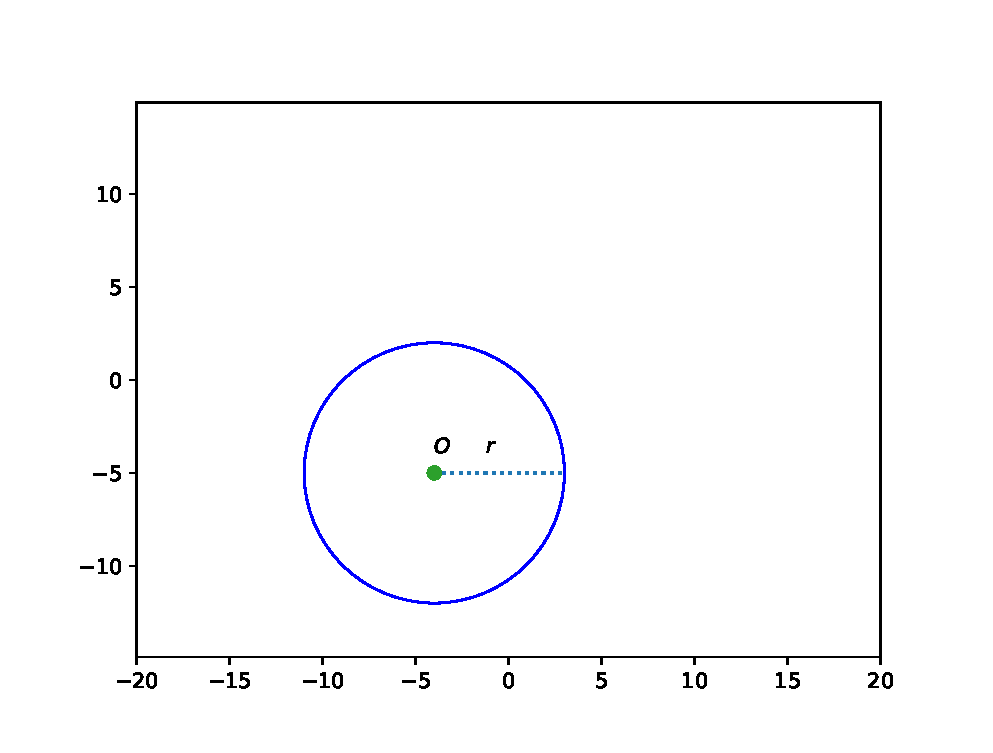
\includegraphics[width=\columnwidth]{./figs/circle_examp/circle.eps}
\caption{Circle generated using python}
\label{fig:circle2_circle_examp}
\end{figure} 

The following Python code generates Fig. \ref{fig:circle2_circle_examp}

\begin{lstlisting}
codes/circle_exam.py
\end{lstlisting}

\end{enumerate}